% This LaTeX was auto-generated from MATLAB code.
% To make changes, update the MATLAB code and export to LaTeX again.

\documentclass{article}

\usepackage[utf8]{inputenc}
\usepackage[T1]{fontenc}
\usepackage{lmodern}
\usepackage{graphicx}
\usepackage{color}
\usepackage{hyperref}
\usepackage{amsmath}
\usepackage{amsfonts}
\usepackage{epstopdf}
\usepackage[table]{xcolor}
\usepackage{matlab}

\usepackage[active,tightpage]{preview}
\renewcommand{\PreviewBorder}{8mm}
\newcommand{\Newpage}{\end{preview}\begin{preview}}

\sloppy
\epstopdfsetup{outdir=./}
\graphicspath{ {./ecen415_ass2_eisendani_images/} }

\title{ECEN 415 \\ Assignment 2 Submission}
\author{Daniel Eisen : 300447549}
\date{\today}

\begin{document}
\begin{preview}
\maketitle

\matlabheadingthree{\textbf{1.}\textit{ A state space system is described by the system matrices}}

\begin{par}
\hfill \break
\end{par}

\begin{matlabcode}
clear;

A = [12.5314, -91.36   , 28.7129, 59.9628; 
     21.316 , -115.6631, 37.5584, 75.0519; 
     13.967 , -53.5817 , 15.4161, 33.4391; 
     20.5222, -123.3107, 42.267 , 79.7156];
 
B = [1.7649, 1.7649; 
     2.8318, 2.8318; 
     2.2353, 2.2353; 
     2.7294, 2.7294];
 
C = [-0.46166, -4.4635, 1.9151, 3.7274;
      1.0853 , -12.82 , 4.5753, 8.3759];
  
D = [0, 0; 
     0, 0];
\end{matlabcode}


\begin{par}
\begin{flushleft}
\textbf{a)}\textit{ If the system begins in a state }$\mathit{\mathbf{x}}\left(0\right)={\left\lbrack 1\;1\;1\;2\right\rbrack }^T$\textit{, use matlab's }\texttt{\textbf{lsim }}\textit{command to plot the response of the system in the time interval }$t\in \left\lbrack 0,10\right\rbrack \;s$\textit{. You should plot the evolution of the system state }$\left(\mathit{\mathbf{x}}\right)$\textit{ and its output}$\left(\mathit{\mathbf{y}}\right)$\textit{as a functions of time.}
\end{flushleft}
\end{par}

\begin{par}
\begin{flushleft}
\textit{Hint: BY default, Matlab will plot the system response for you when you use }\texttt{\textbf{lsim}}\textit{, but make sure that you can extract the required signal from }\texttt{\textbf{lsim}}\textit{ so that you can do other things with them (including plotting them yourself). We will need this later.}
\end{flushleft}
\end{par}

\begin{matlabcode}
sys = ss(A,B,C,D);           %create system
x0 = [1; 1; 1; 2];           %initial state
t = 0:0.01:10;               %time vector
u = zeros(length(t),2);      %inputs for all t, 2 wide
[Y,T,X] = lsim(sys,u,t,x0);  %extract outputs, t vect, states

figure();
plot(T,X);
title("System State");
legend("X_1","X_2","X_3","X_4");
xlabel('t[s]')
grid on;
\end{matlabcode}
\begin{center}
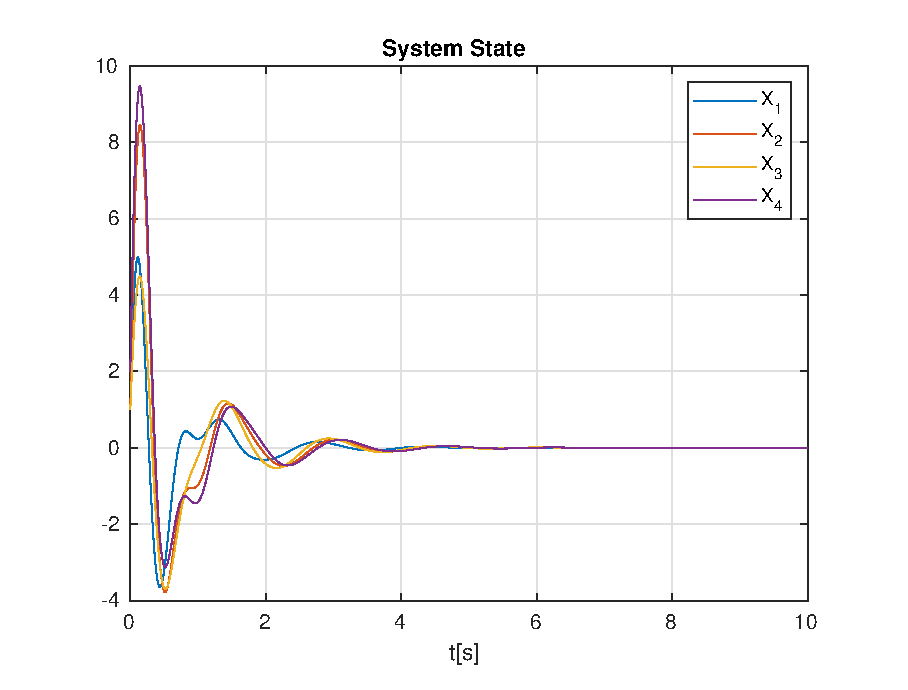
\includegraphics[width=\maxwidth{57.90265930757652em}]{figure_0.eps}
\end{center}
\begin{matlabcode}
figure();
plot(T,Y);
title("Output");
legend("Y_1","Y_2");
xlabel('t[s]')
grid on;
\end{matlabcode}
\begin{center}
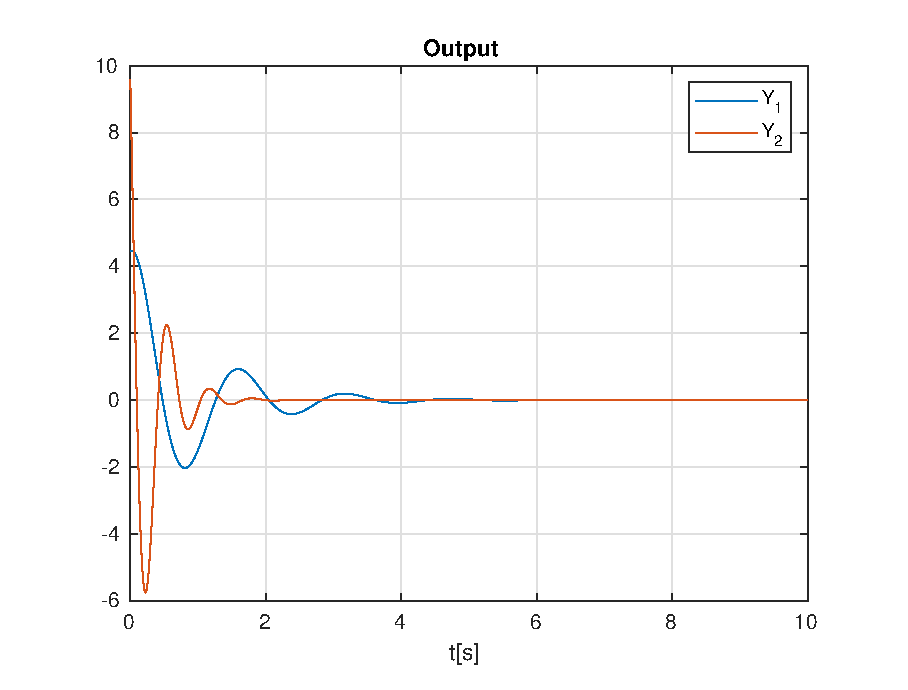
\includegraphics[width=\maxwidth{57.90265930757652em}]{figure_1.eps}
\end{center}


\begin{par}
\begin{flushleft}
\textbf{b}\underline{\textbf{)}}\textit{ Replicate the results from above using the matrix exponential to evolve the state, rather than }\texttt{\textbf{lsim}}\textit{.}
\end{flushleft}
\end{par}

\begin{matlabcode}
Xe = [];                    %State history 
Ye = [];                    %Output history 
for t_ = t                  %reuse previous t vector
    xe = expm(A*t_)*x0;     %compute phi*x_0
    ye = C*xe + D*[0; 0];   %output
    
    %append to history
    Xe = [Xe; xe'];
    Ye = [Ye; ye'];
end

figure();
plot(t',Xe);
title("System State");
legend("X_1","X_2","X_3","X_4");
xlabel('t[s]')
grid on;
\end{matlabcode}
\begin{center}
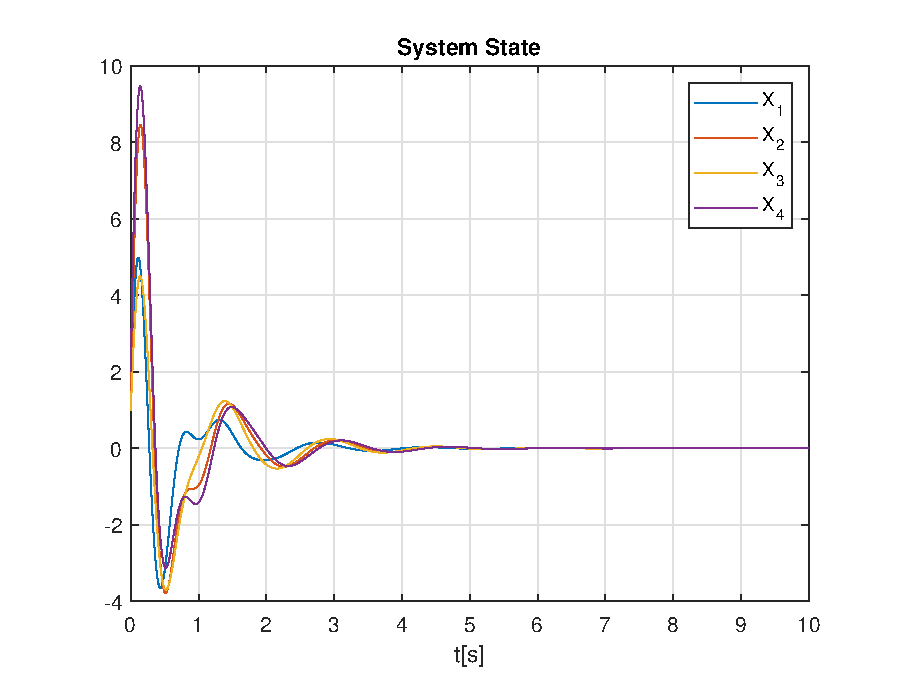
\includegraphics[width=\maxwidth{57.90265930757652em}]{figure_2.eps}
\end{center}
\begin{matlabcode}
figure();
plot(t',Ye);
title("Output");
legend("Y_1","Y_2");
xlabel('t[s]')
grid on;
\end{matlabcode}
\begin{center}
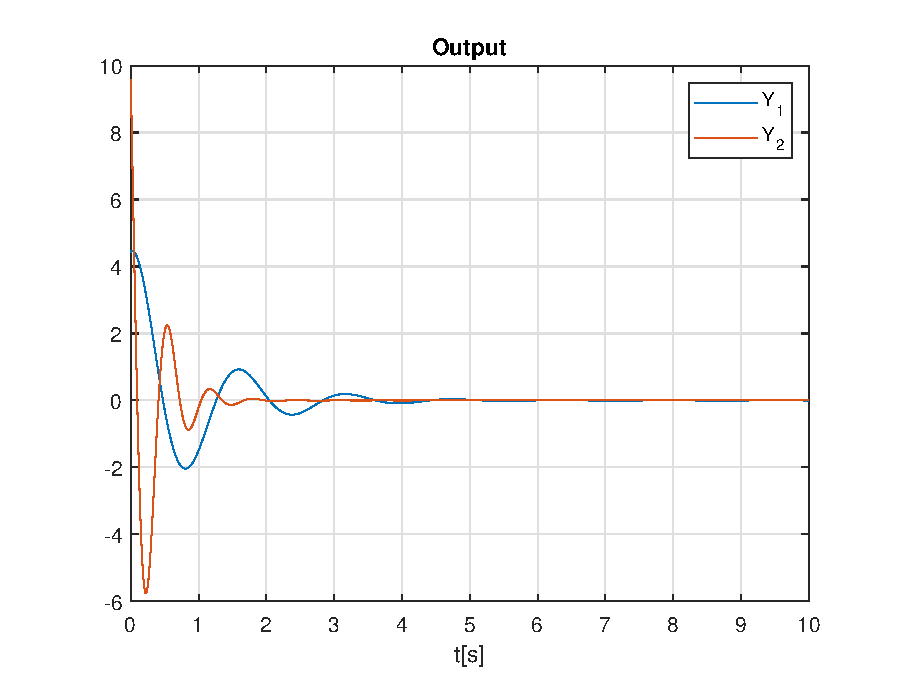
\includegraphics[width=\maxwidth{57.90265930757652em}]{figure_3.eps}
\end{center}


\begin{par}
\begin{flushleft}
\textbf{c)}\textit{ Use }\texttt{\textbf{lsim}}\texttt{\textit{ }}\textit{to plot the response of the system to the input signal }$\mathit{\mathbf{u}}={\left\lbrack u_1 \;\;\;\;u_2 \right\rbrack }^T$\textit{with:}
\end{flushleft}
\end{par}

\begin{par}
$$\begin{array}{l}
u_1 =u\left(t-1\right)\\
u_2 =2u\left(t-5\right)
\end{array}$$
\end{par}

\begin{par}
\begin{flushleft}
\textit{for }$u$\textit{ the (Heaviside) unit step function.}
\end{flushleft}
\end{par}

\begin{matlabcode}
u_ = zeros(length(t),2);   %generate empty input
u_(t>=1,1) = 1;            %piecewise steps at t=1 and t=5
u_(t>=5,2) = 2;

[Y_,T_,X_] = lsim(sys,u_,t,x0);

figure();
plot(T_,X_);
hold on
plot(t,u_,'Color',[0.5,0.5,0.5]);
hold off
title("System State");
legend("X_1","X_2","X_3","X_4");
xlabel('t[s]')
grid on;
\end{matlabcode}
\begin{center}
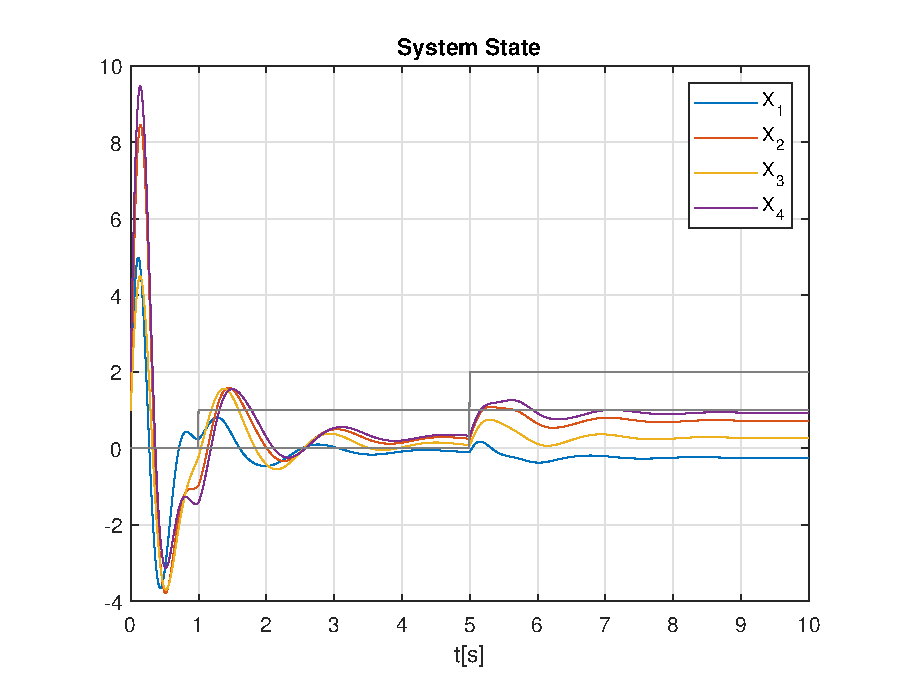
\includegraphics[width=\maxwidth{57.90265930757652em}]{figure_4.eps}
\end{center}
\begin{matlabcode}
figure();
plot(T_,Y_);
hold on
plot(t,u_,'Color',[0.5,0.5,0.5]);
hold off
title("Output");
legend("Y_1","Y_2");
xlabel('t[s]')
grid on;
\end{matlabcode}
\begin{center}
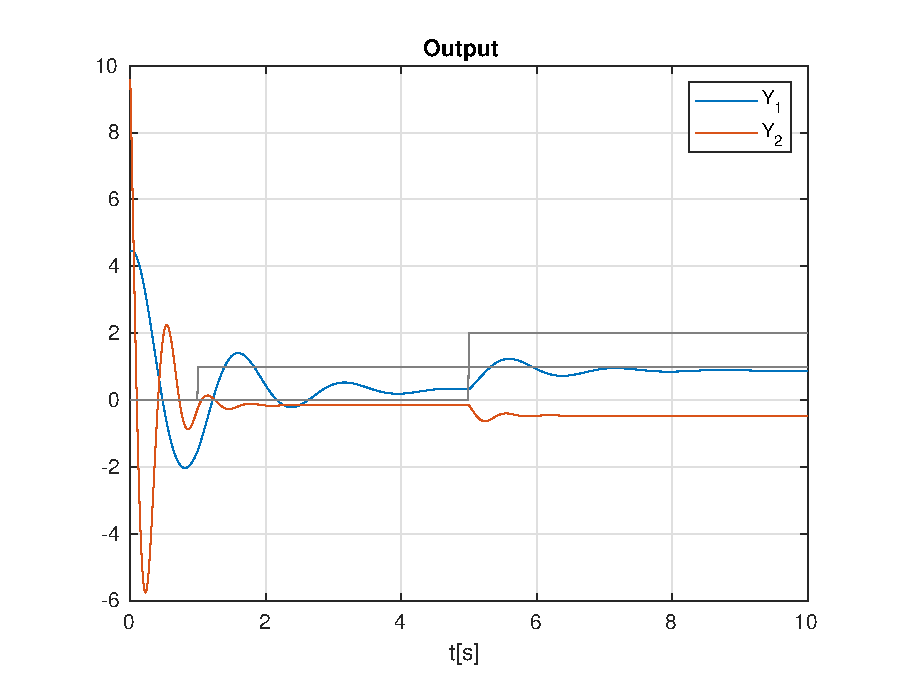
\includegraphics[width=\maxwidth{57.90265930757652em}]{figure_5.eps}
\end{center}


\begin{par}
\begin{flushleft}
\textbf{d)}\textit{ Use }\texttt{\textbf{c2d}}\texttt{\textit{ }}\textit{to discretise the system with an appropriate sampling frequency and use }\texttt{\textbf{lsim}}\texttt{\textit{ }}\textit{to plot the response of the discrete time system.}
\end{flushleft}
\end{par}

\begin{matlabcode}
ts=0.05;                    %sampling time
zyz = c2d(sys,ts);          %discrete system
tz = 0:ts:10;               %match t vector and input
uz = zeros(length(tz),2);

[Yz,Tz,Xz] = lsim(zyz,uz,tz,x0);

figure();
stairs(Tz,Xz);
title("System State");
legend("Xz_1","Xz_2","Xz_3","Xz_4");
xlabel('t[s]')
grid on;
\end{matlabcode}
\begin{center}
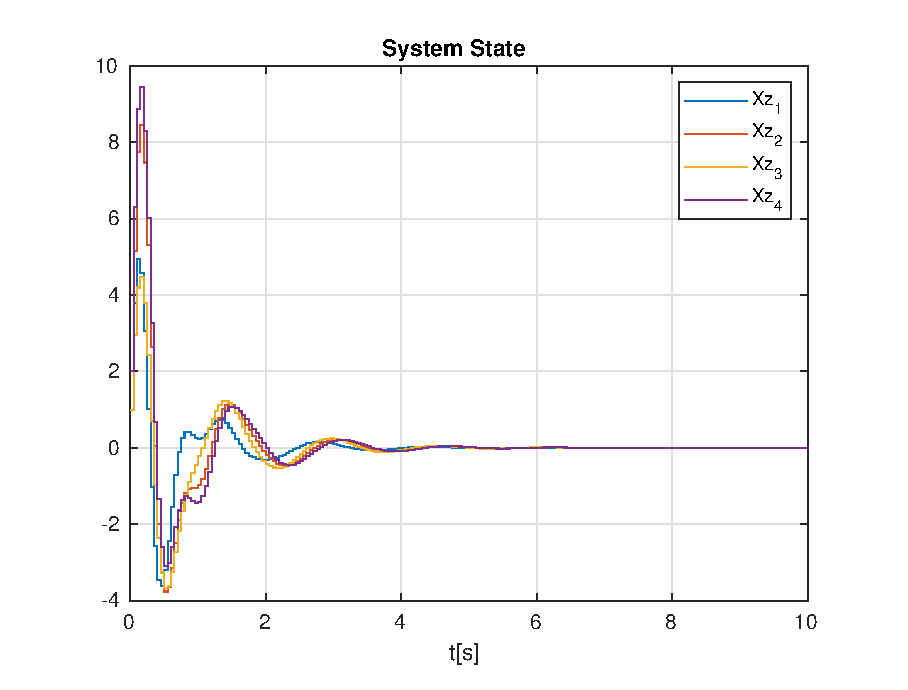
\includegraphics[width=\maxwidth{57.90265930757652em}]{figure_6.eps}
\end{center}
\begin{matlabcode}
figure();
stairs(Tz,Yz);
title("Output");
legend("Yz_1","Yz_2");
xlabel('t[s]')
grid on;
\end{matlabcode}
\begin{center}
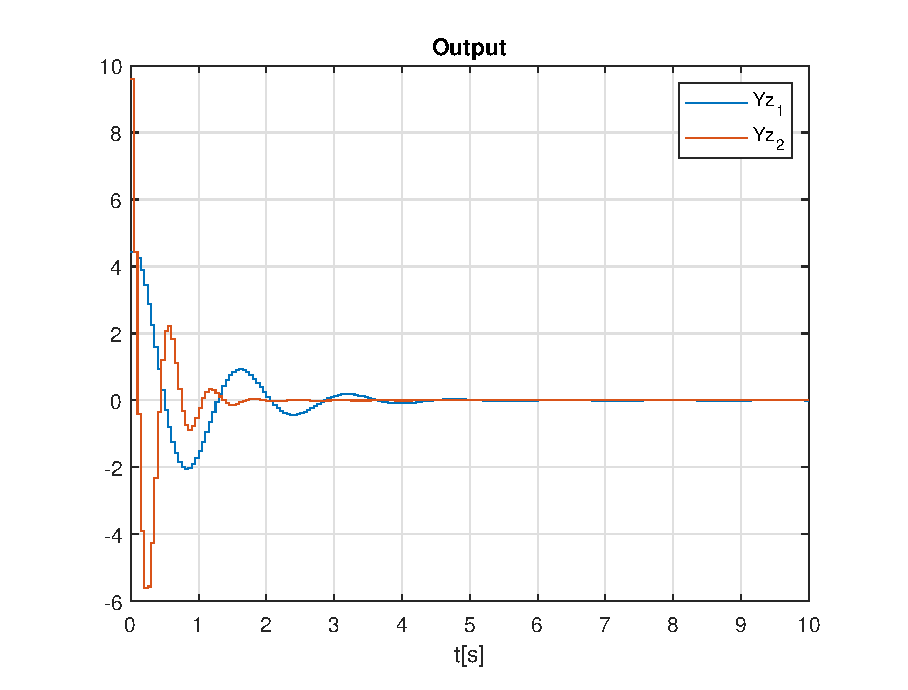
\includegraphics[width=\maxwidth{57.90265930757652em}]{figure_7.eps}
\end{center}

\begin{par}
\begin{flushleft}
\textbf{e)}\textit{ Vary the sampling period and describe the effect on the output.}
\end{flushleft}
\end{par}

\begin{matlabcode}
figure();
for ts = [0.5 0.15 0.05]     %varied ts's 
    zyz = c2d(sys,ts);
    tz = 0:ts:10;
    uz = zeros(length(tz),2);

    [Yz,Tz,Xz] = lsim(zyz,uz,tz,x0);
    stairs(tz, Yz(:,1))
    hold on
end
plot(T,Y(:,1))  %plot the original system
title('Varied Sampling Period of Discretised System')
legend("ts=0.5","ts=0.15", "ts=0.05", "continuous");
xlim([0.00 3])
ylim([-4 6])
xlabel('t[s]')
ylabel('Y_1')
grid on
hold off
\end{matlabcode}
\begin{center}
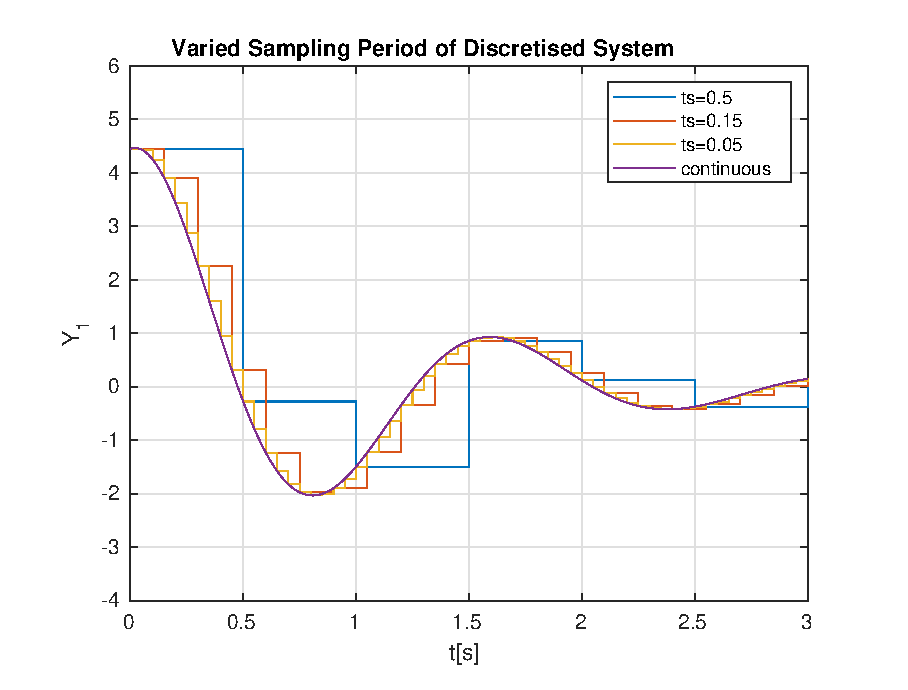
\includegraphics[width=\maxwidth{57.90265930757652em}]{figure_8.eps}
\end{center}

\begin{par}
\begin{flushleft}
Varying the sampling time most noticeably affects the resolution of the computed signals. Hence showing to accurately represent a given system an appropriate \texttt{\textbf{ts}} must be chosen to prevent aliasing of the given states/outputs, though any given point is still accurate.
\end{flushleft}
\end{par}


\begin{par}
\begin{flushleft}
\textbf{f)} \textit{Find the time response for the discrete time system of there is no input and initial conditions of}$\mathit{\mathbf{x}}={\left\lbrack 1\;1\;1\;2\right\rbrack }^T$\textit{. Determine this response using powers of}$\mathit{\mathbf{A}}$\textit{directly (ie, do not use }\texttt{\textbf{lsim}}\textit{).}
\end{flushleft}
\end{par}

\begin{matlabcode}
%compute discrete A matrix
Ad = expm(ts*A);                    

Xzp = [];
Yzp = [];

for tz_ = tz
    %compute next state and scale by sampling time 
    xzp = real((Ad^(tz_/ts))*x0);   
    yzp = C*xzp;
    
    Xzp = [Xzp; xzp'];
    Yzp = [Yzp; yzp'];
end

figure();
stairs(tz,Xzp);
title("System State");
legend("Xz_1","Xz_2","Xz_3","Xz_4");
xlabel('t[s]')
grid on;
\end{matlabcode}
\begin{center}
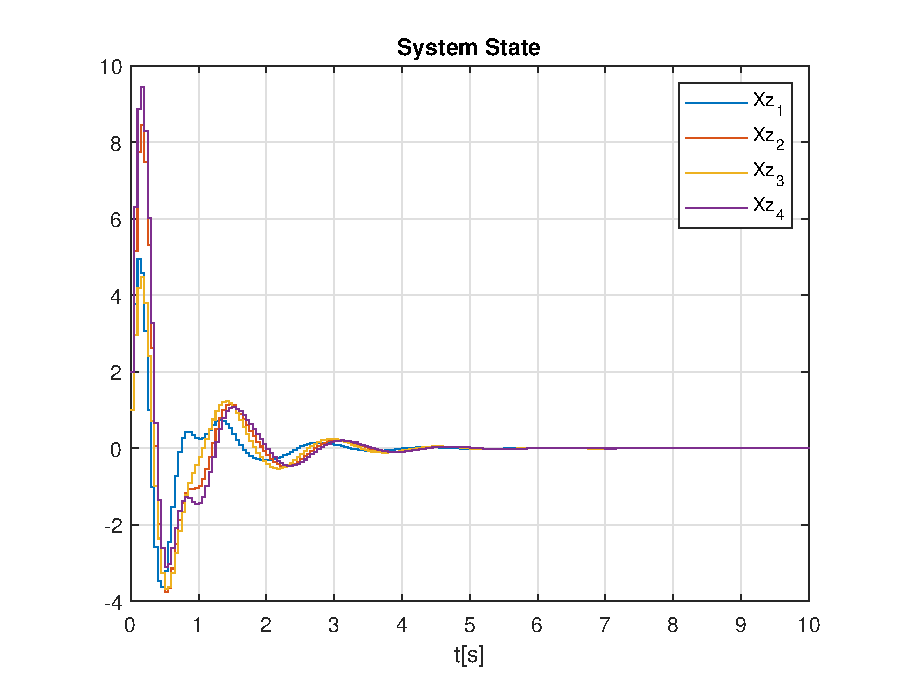
\includegraphics[width=\maxwidth{57.90265930757652em}]{figure_9.eps}
\end{center}
\begin{matlabcode}
figure();
stairs(tz,Yzp);
title("Output");
legend("Yz_1","Yz_2");
xlabel('t[s]')
grid on;
\end{matlabcode}
\begin{center}
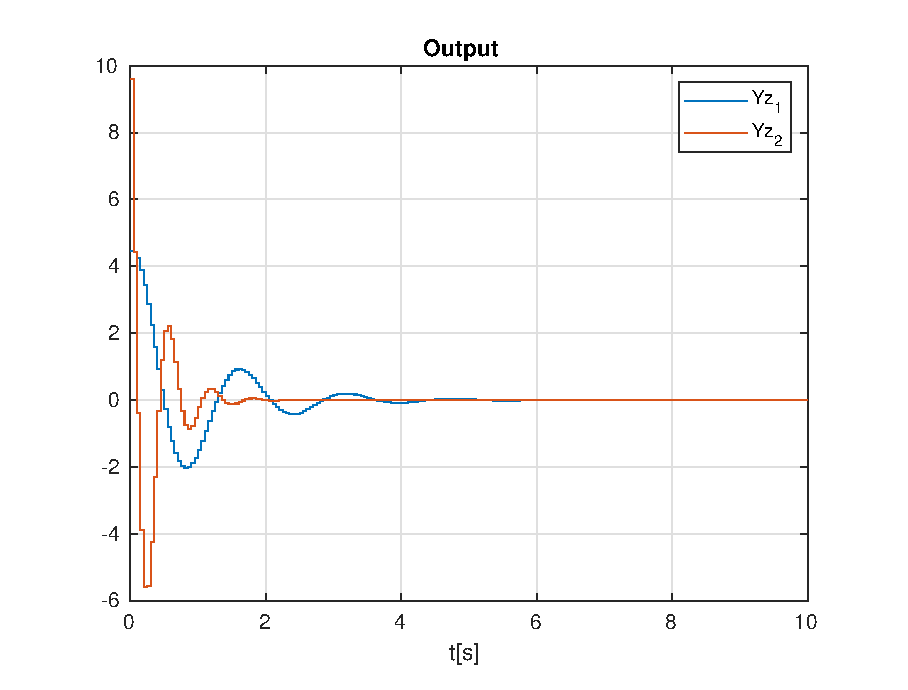
\includegraphics[width=\maxwidth{57.90265930757652em}]{figure_10.eps}
\end{center}


\matlabheadingthree{2. The phase-shift oscillator circuit shown in figure 1 can be described by the coupled differential equations}

\begin{par}
$$\begin{array}{l}
{\dot{v} }_a =-\frac{2v_a }{\textrm{RC}}+\frac{v_b }{\textrm{RC}}-\frac{R_2 }{R_1 }\frac{v_c }{\textrm{RC}}\\
{\dot{v} }_b =\frac{v_a }{\textrm{RC}}-\frac{2v_b }{\textrm{RC}}+\frac{v_c }{\textrm{RC}}\\
{\dot{v} }_c =\frac{v_b }{\textrm{RC}}-\frac{v_c }{\textrm{RC}}-\frac{v_c }{R_1 C}
\end{array}$$
\end{par}

\matlabheadingthree{where $v_a$, $v_b$ and $v_c$ are the voltages after the three successive $\textrm{RC}$ stages.}

\begin{par}
\begin{center}
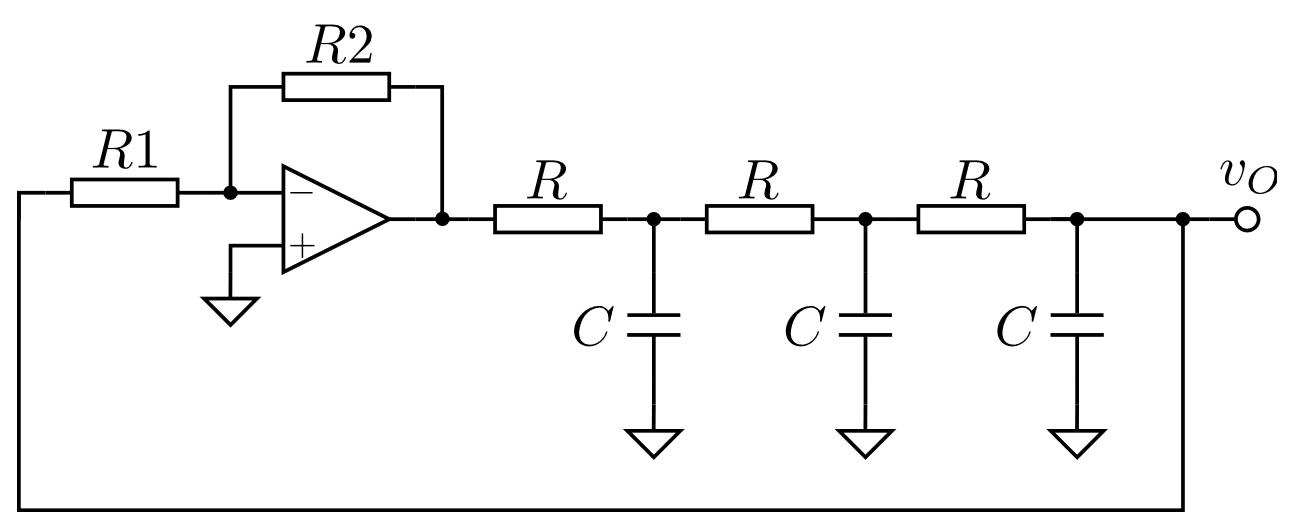
\includegraphics[width=\maxwidth{61.01354741595585em}]{image_0}
\end{center}
\end{par}

\begin{par}
\begin{center}
Figure 1: An unbuffered phase-shift oscillator
\end{center}
\end{par}


\vspace{1em}
\begin{par}
\begin{flushleft}
\textbf{a) }\textit{Write a state space representation for the system.}
\end{flushleft}
\end{par}


\vspace{1em}
\begin{par}
$$\left\lbrack \begin{array}{c}
{\dot{v} }_a \\
{\dot{v} }_b \\
{\dot{v} }_c 
\end{array}\right\rbrack =\left\lbrack \begin{array}{ccc}
-\frac{2}{\textrm{RC}} & \frac{1}{\textrm{RC}} & -\frac{R_2 }{R_1 }\frac{1}{\textrm{RC}}\\
\frac{1}{\textrm{RC}} & -\frac{2}{\textrm{RC}} & \frac{1}{\textrm{RC}}\\
0 & \frac{1}{\textrm{RC}} & -\frac{1}{\textrm{RC}}-\frac{1}{R_1 C}
\end{array}\right\rbrack \left\lbrack \begin{array}{c}
v_a \\
v_b \\
v_c 
\end{array}\right\rbrack$$
\end{par}

\begin{par}
$$v_o =\left\lbrack \begin{array}{ccc}
0 & 0 & 1
\end{array}\right\rbrack \left\lbrack \begin{array}{c}
v_a \\
v_b \\
v_c 
\end{array}\right\rbrack$$
\end{par}

\begin{par}
$$A=$$$$\left\lbrack \begin{array}{ccc}
-\frac{2}{\textrm{RC}} & \frac{1}{\textrm{RC}} & -\frac{R_2 }{R_1 }\frac{1}{\textrm{RC}}\\
\frac{1}{\textrm{RC}} & -\frac{2}{\textrm{RC}} & \frac{1}{\textrm{RC}}\\
0 & \frac{1}{\textrm{RC}} & -\frac{1}{\textrm{RC}}-\frac{1}{R_1 C}
\end{array}\right\rbrack ,\;C=\left\lbrack \begin{array}{ccc}
0 & 0 & 1
\end{array}\right\rbrack$$
\end{par}

\begin{par}
\begin{flushleft}
\textbf{b) }\textit{The ratio }$\frac{\textrm{R2}}{\textrm{R1}}\approx 30$\textit{ matters if the oscillator is to maintain sustained oscillations.}
\end{flushleft}
\end{par}

\begin{par}
\begin{flushleft}
\textit{Find the value for this ratio that correctly induces oscillation, making sure that you explain your process.}
\end{flushleft}
\end{par}

\begin{par}
\begin{flushleft}
\textit{Hint: You could solve this problem analytically, but don’t!}
\end{flushleft}
\end{par}

\begin{par}
\begin{flushleft}
\textit{Hint: You should choose some convenient values for R and C, given that the nominal oscillation angular frequency is }$\omega_0 =\frac{1}{\sqrt{6}\textrm{RC}}$ .
\end{flushleft}
\end{par}


\vspace{1em}
\begin{par}
\begin{flushleft}
\textbf{Ans.} The eigenvalues of the $A$ matrix correspond to the poles of the system. So to find the point of sustained oscillations, we are looking for purely imaginary poles, e.g. $0\pm 1i$.
\end{flushleft}
\end{par}

\begin{par}
\begin{flushleft}
To find this, R, R1, C were set and R2 swept to find the purely imaginary dominant poles.
\end{flushleft}
\end{par}

\begin{matlabcode}
clear;

r=1000;
r1=r;
c=1e-3;

C=[0, 0, 1];
B=[];
D=[];

res=[];
for r2 = 1000:10:100000     %sweep R2 values
    A=[-(2/(r*c)), 1/(r*c), -(r2/r1)*(1/(r*c));
        1/(r*c)  ,-2/(r*c),  1/(r*c)          ;
        0        ,1/(r*c), -(1/(r*c))-(1/(r1*c))];
    res = [res; [r2,eig(A)']];
    if real(res(end,3)) == 0 %check zero real
        r2
        ratio = r2/r1
        eig(A)
    end
end
\end{matlabcode}
\begin{matlaboutput}
r2 = 56000
ratio = 56
ans = 3x1 complex    
  -6.0000 + 0.0000i
   0.0000 + 3.1623i
   0.0000 - 3.1623i

\end{matlaboutput}
\begin{matlabcode}
r2 = ratio*r1;
figure();
pos_0 = find(real(res(:,3))==0);
plot(real(res(:,1)), abs(real(res(:,3))),
    ...'*-','MarkerEdgeColor','red','MarkerIndices', pos_0)
text(real(res(pos_0,1))-5000, abs(real(res(pos_0,3))-0.1),
    ...num2str(r2))
xlabel('R_2')
ylabel('|Re(\lambda_2)|')
title('R2 Sweep')
\end{matlabcode}
\begin{center}
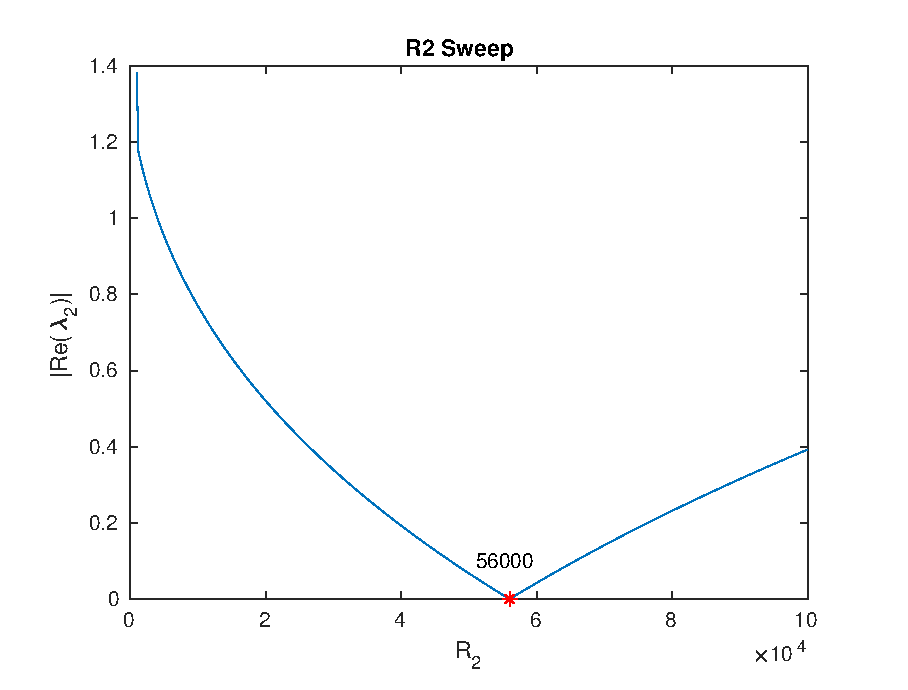
\includegraphics[width=\maxwidth{57.90265930757652em}]{figure_11.eps}
\end{center}

\begin{par}
\begin{flushleft}
Theis gives a R2/R1 ratio of 56 for R=R1=1000
\end{flushleft}
\end{par}


\vspace{1em}
\begin{par}
\begin{flushleft}
\textbf{c) }\textit{Determine the oscillation frequency of the circuit using the state space model.}
\end{flushleft}
\end{par}

\begin{matlabcode}

 A=[-(2/(r*c)) , 1/(r*c), -(r2/r1)*(1/(r*c));
        1/(r*c),-2/(r*c),   1/(r*c)         ;
        0      , 1/(r*c), -(1/(r*c))-(1/(r1*c))];
poles = eig(A)
\end{matlabcode}
\begin{matlaboutput}
poles = 3x1 complex    
  -6.0000 + 0.0000i
   0.0000 + 3.1623i
   0.0000 - 3.1623i

\end{matlaboutput}
\begin{matlabcode}

w = imag(poles(2)) %rad/s
\end{matlabcode}
\begin{matlaboutput}
w = 3.1623
\end{matlaboutput}
\begin{matlabcode}

f = w/(2*pi) %Hz
\end{matlabcode}
\begin{matlaboutput}
f = 0.5033
\end{matlaboutput}

\begin{par}
\begin{flushleft}
\textbf{d) }\textit{Simulate the operation of the oscillator to show that it works as you might expect.}
\end{flushleft}
\end{par}

\begin{par}
\begin{flushleft}
\textit{Hint: Think about the initial conditions for the simulation.}
\end{flushleft}
\end{par}


\vspace{1em}
\begin{par}
\begin{flushleft}
\textbf{Ans: }By using the the eigenvector(s) of the oscillatry pole are an initial state we can observer the sustained osculations at the above computed frequency.
\end{flushleft}
\end{par}

\begin{matlabcode}
sys = ss(A,B,C,D);
[V,wc] = eig(A);
x0 = V(:,2);
t = 0:0.01/f:4/f;
[Y,T,X] = lsim(sys,[],t,x0);

figure();
plot(T,real(X));
title("System State");
legend("v_a","v_b","v_c");
xlabel('t[s]')
grid on;
\end{matlabcode}
\begin{center}
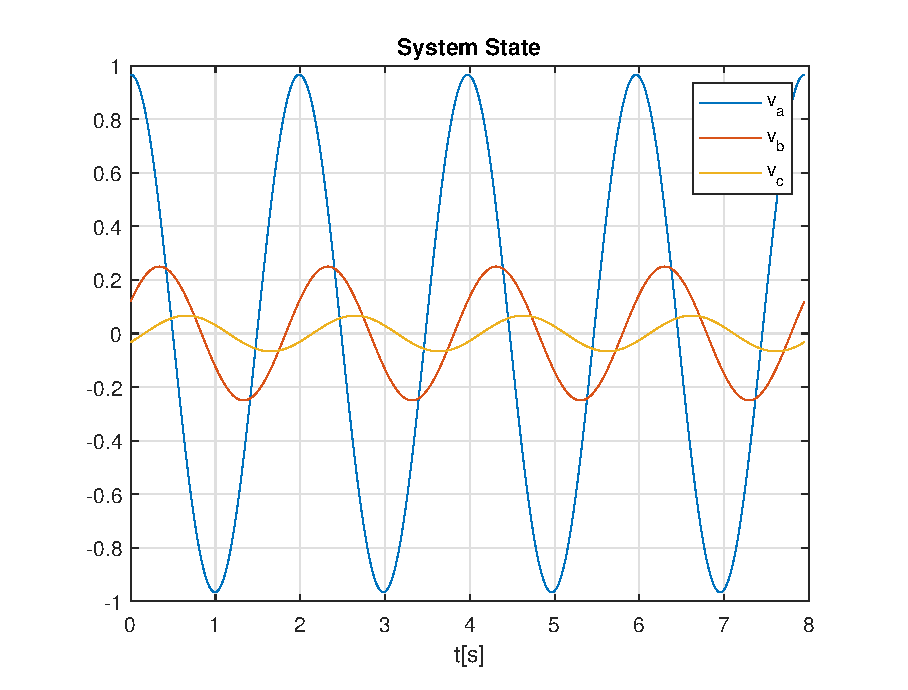
\includegraphics[width=\maxwidth{57.90265930757652em}]{figure_12.eps}
\end{center}
\begin{matlabcode}
figure();
plot(T,real(Y));
title("Output");
legend("v_o");
xlabel('t[s]')
grid on;
\end{matlabcode}
\begin{center}
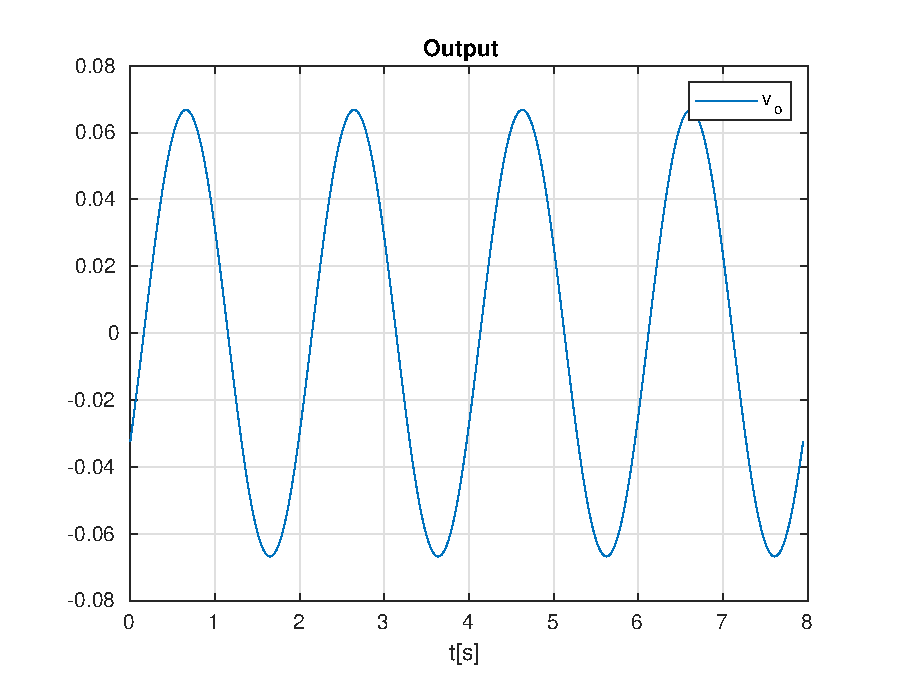
\includegraphics[width=\maxwidth{57.90265930757652em}]{figure_13.eps}
\end{center}


\matlabheadingthree{\textit{3. You need to design a simple open loop "controller" that causes a rocket to pitch }${10}^{\circ }$\textit{ clockwise by the end of the first 15 seconds of flight. The idea is nominally to let the rocket ascend for the first five seconds and then pitch over at approximately }$1^{\circ } /s$\textit{ for the remaining 10 seconds. The main rocket engine is at full burn throughout the period.}}

\matlabheadingthree{\textit{A continuous time, nonlinear model for the rocket is as described below. Simulation code for the complete nonlinear system is available on the course website.}}

\matlabheadingthree{\textit{In this question you will investigate the approximations due to linearisation of the system, as well as examining the time evolution of the system.}}


\vspace{1em}
\begin{par}
\begin{flushleft}
Let the state vector be defined as follows:
\end{flushleft}
\end{par}

\begin{par}
\begin{flushleft}
                        $x_1 \equiv$ Rocket’s altitude (positive upwards) $\left\lbrack m\right\rbrack$
\end{flushleft}
\end{par}

\begin{par}
\begin{flushleft}
                        $x_2 \equiv$ Rocket’s vertical velocity (positive upwards) $m/s$
\end{flushleft}
\end{par}

\begin{par}
\begin{flushleft}
                        $x_3 \equiv$ Rocket’s horizontal position relative to launch site $\left\lbrack m\right\rbrack$
\end{flushleft}
\end{par}

\begin{par}
\begin{flushleft}
                        $x_4 \equiv$ Rocket’s horizontal ground speed $\left\lbrack m/s\right\rbrack$
\end{flushleft}
\end{par}

\begin{par}
\begin{flushleft}
                        $x_5 \equiv$ Rocket’s angle from vertical $\left\lbrack \circ \right\rbrack$
\end{flushleft}
\end{par}

\begin{par}
\begin{flushleft}
                        $x_6 \equiv$ Rocket’s angular velocity $\left\lbrack \circ /s\right\rbrack$
\end{flushleft}
\end{par}

\begin{par}
\begin{flushleft}
                        $x_7 \equiv$ Fuel load $\left\lbrack \textrm{kg}\right\rbrack$
\end{flushleft}
\end{par}

\begin{par}
\begin{flushleft}
and the input vector is:
\end{flushleft}
\end{par}

\begin{par}
\begin{flushleft}
                        $u_1 \equiv$ Main engine force (positive upwards) $\left\lbrack N\right\rbrack$
\end{flushleft}
\end{par}

\begin{par}
\begin{flushleft}
                        $u_2 \equiv$ Orientation thruster force (positive rotates the rocket clockwise) $\left\lbrack N\right\rbrack$
\end{flushleft}
\end{par}

\begin{par}
\begin{flushleft}
The initial state is:
\end{flushleft}
\end{par}

\begin{par}
\begin{flushleft}
                        $x\left(0\right)={\left\lbrack \begin{array}{ccccccc}
0 & 0 & 0 & 0 & 0 & 0 & 1000
\end{array}\right\rbrack }^T$,
\end{flushleft}
\end{par}

\begin{par}
\begin{flushleft}
which is to say that before launch it is stationary at the origin, with 1000 kg of fuel on board.
\end{flushleft}
\end{par}

\begin{par}
\begin{flushleft}
The rocket’s state evolves according to the following set of non-linear equations.
\end{flushleft}
\end{par}

\begin{par}
$$\left\lbrace \begin{array}{l}
{\dot{x} }_1 =x_2 \\
{\dot{x} }_2 =g-c_d x_2^2 +\frac{\cos \left(x_5 \right)}{\left(M+x_7 \right)}u_1 \\
{\dot{x} }_3 =x_4 \\
{\dot{x} }_4 =-\frac{\sin \left(x_5 \right)}{\left(M+x_7 \right)}u_1 \\
{\dot{x} }_5 =x_6 \\
{\dot{x} }_6 =\frac{k}{J+L^2 x_7 }\\
{\dot{x} }_7 =-\frac{1}{\eta }\left(u_1 +u_2 \right)
\end{array}\right.$$
\end{par}

\begin{par}
\begin{center}
where,$\left\lbrace \begin{array}{l}
g=9\ldotp 8\;\textrm{the}\;\textrm{acceleration}\;\textrm{due}\;\textrm{to}\;\textrm{gravity}\;\left\lbrack {\textrm{ms}}^{-2} \right\rbrack \\
c_d =2\times {10}^{-3} \;\textrm{is}\;\textrm{the}\;\textrm{coefficient}\;\textrm{of}\;\textrm{drag}\;\left\lbrack {\textrm{Nm}}^{-2} s^2 \right\rbrack \\
M=1000\;\textrm{is}\;\textrm{the}\;\textrm{mass}\;\textrm{of}\;\textrm{the}\;\textrm{empty}\;\textrm{rocket}\;\left\lbrack \textrm{kg}\right\rbrack \\
J=20,000\;\textrm{is}\;\textrm{the}\;\textrm{moment}\;\textrm{of}\;\textrm{inertia}\;\textrm{of}\;\textrm{empty}\;\textrm{rocket}\;\left\lbrack \textrm{kg}\;m^2 \right\rbrack \\
L=5\;\textrm{is}\;\textrm{the}\;\textrm{distance}\;\textrm{between}\;\textrm{the}\;\textrm{rocket’s}\;\textrm{centre}\;\textrm{of}\;\textrm{mass}\;\textrm{and}\;\textrm{the}\;\textrm{centre}\;\textrm{of}\;\textrm{the}\;\textrm{fuel}\;\textrm{load}\;\left\lbrack m\right\rbrack \\
\eta =1000\;\textrm{is}\;\textrm{the}\;\textrm{efficiency}\;\textrm{of}\;\textrm{the}\;\textrm{fuel}\;\left\lbrack \textrm{Ns}/\textrm{kg}\right\rbrack \\
k=6\;\textrm{is}\;\textrm{the}\;\textrm{distance}\;\textrm{between}\;\textrm{the}\;\textrm{rotation}\;\textrm{thruster}\;\textrm{and}\;\textrm{the}\;\textrm{centre}\;\textrm{of}\;\textrm{mass}\;\left\lbrack m\right\rbrack 
\end{array}\right.$
\end{center}
\end{par}

\begin{par}
\begin{flushleft}
(Note that these quantities may not make physical sense; they are constructed to make an interesting exercise. In addition, the model doesn’t attempt to capture all of the non-linear effects. As an example $L$ should most likely change as the fuel load is depleted.)
\end{flushleft}
\end{par}

\begin{par}
\begin{flushleft}
Hints:
\end{flushleft}
\end{par}

\begin{par}
\begin{flushleft}
1. The non-linear simulation code calculates the rocket’s trajectory in time chunks of length \texttt{\textbf{dt}}. The control input $\mathit{\mathbf{u}}$ is calculated only once per time chunk. If you decrease \texttt{\textbf{dt}}\texttt{ }the ODE solver may be more accurate, and as a side effect you can calculate $\mathit{\mathbf{u}}$ more frequently (and vice versa). This may be useful for debugging, but your final solution will be marked with \texttt{\textbf{dt=1}}. However, for this assignment you need not change $\mathit{\mathbf{u}}$ anyway, so there is little to be gained by changing $\textrm{dt}$.
\end{flushleft}
\end{par}

\begin{par}
\begin{flushleft}
2. The sample code includes a symbolic model \texttt{\textbf{f\_sym}}\texttt{ }that should be useful in finding the linear approximations of the system, but you may choose to find it by hand. To implement the linearised systems, you should find a linear model and then rewrite the simulation section of the code to use \texttt{\textbf{lsim}}\texttt{ }rather than \texttt{\textbf{ode45}}.
\end{flushleft}
\end{par}


\begin{par}
\begin{flushleft}
\textbf{a)} \textbf{[5 marks]}\textit{ Use the non-linear model to devise a nominal control signal }$\mathit{\mathbf{u}}$\textit{. You should assume that }$u_1$\textit{ is a constant throughout the 15 seconds of flight, such that there is no remaining fuel after that time. You should then choose }$u_2$\textit{ to effect the required pitch-over manoeuvre.}
\end{flushleft}
\end{par}

\begin{par}
\begin{flushleft}
\textit{You don’t need to be too fussy about this; just devise something simple that you can use for comparison in the following parts of the question.}
\end{flushleft}
\end{par}

\begin{par}
\begin{flushleft}
\textit{Hint: Your code to set }$\mathit{\mathbf{u}}$\textit{ should go in the section marked with asterisks. The simulation will not do much until you out something in this section.}
\end{flushleft}
\end{par}


\vspace{1em}
\begin{par}
\begin{flushleft}
\textbf{Ans.} $\left\lbrack \begin{array}{c}
u_1 \\
u_2 
\end{array}\right\rbrack =\left\lbrack \begin{array}{c}
42000\\
1198\ldotp 75
\end{array}\right\rbrack \to \mathrm{final}\;\mathrm{angle}:10\ldotp 0000$
\end{flushleft}
\end{par}

\begin{matlabcode}
clear;
constant_u1 = 42000;
final_u2 = 1198.75;
figure();
run("q3_nonlinear_sim.m");
\end{matlabcode}
\begin{center}
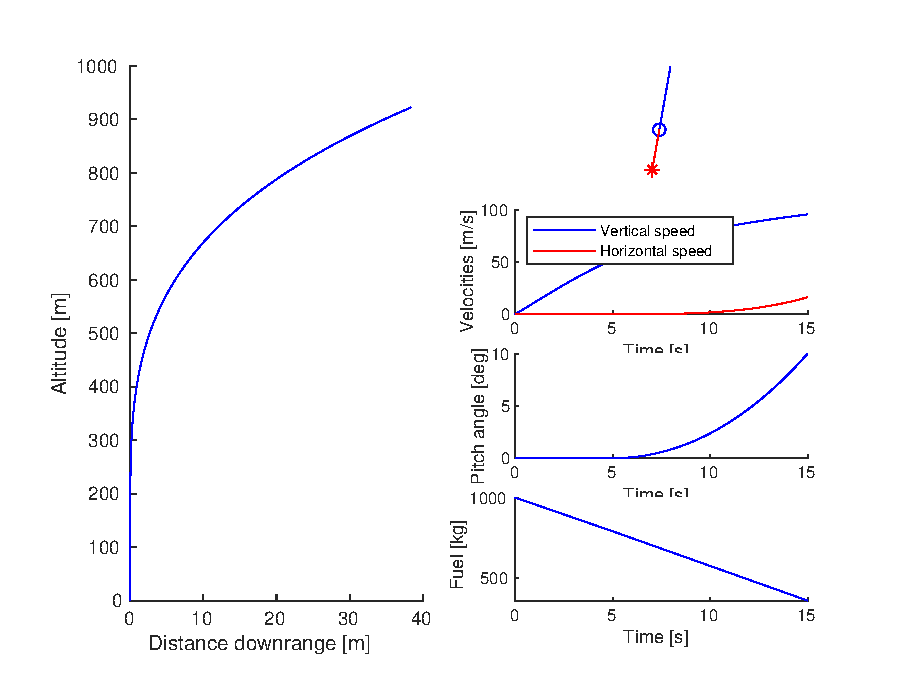
\includegraphics[width=\maxwidth{57.90265930757652em}]{figure_14.eps}
\end{center}
\begin{matlaboutput}
final_angle = 10.0000
\end{matlaboutput}


\begin{par}
\begin{flushleft}
\textbf{b) [2 marks]} \textit{What is the maximum acceleration seen by the rocket during the launch?}
\end{flushleft}
\end{par}

\begin{matlabcode}
T = unique(t_store);
clean_X = unique(x_store,"rows");

v_y = clean_X(:,2);
v_x = clean_X(:,4);

a_y = diff(v_y)./diff(T);
a_x = diff(v_x)./diff(T);
a = sqrt((a_x.^2)+(a_y.^2));

[a_max, max_i] = max(a)
\end{matlabcode}
\begin{matlaboutput}
a_max = 11.3965
max_i = 57
\end{matlaboutput}
\begin{matlabcode}

figure();
% subplot(111);
plot(T(2:end),a_y,T(2:end),a_x,T(2:end),a,
    ...'*-','MarkerEdgeColor','red','MarkerIndices', max_i);
legend({'Vertical Acceleration','Horizontal Acceleration',
    ...'Total Acceleration'})
text(T(max_i-25), a(max_i)-0.5, num2str(a_max))
xlabel('t[s]')
ylabel('ms^{-2}')
\end{matlabcode}
\begin{center}
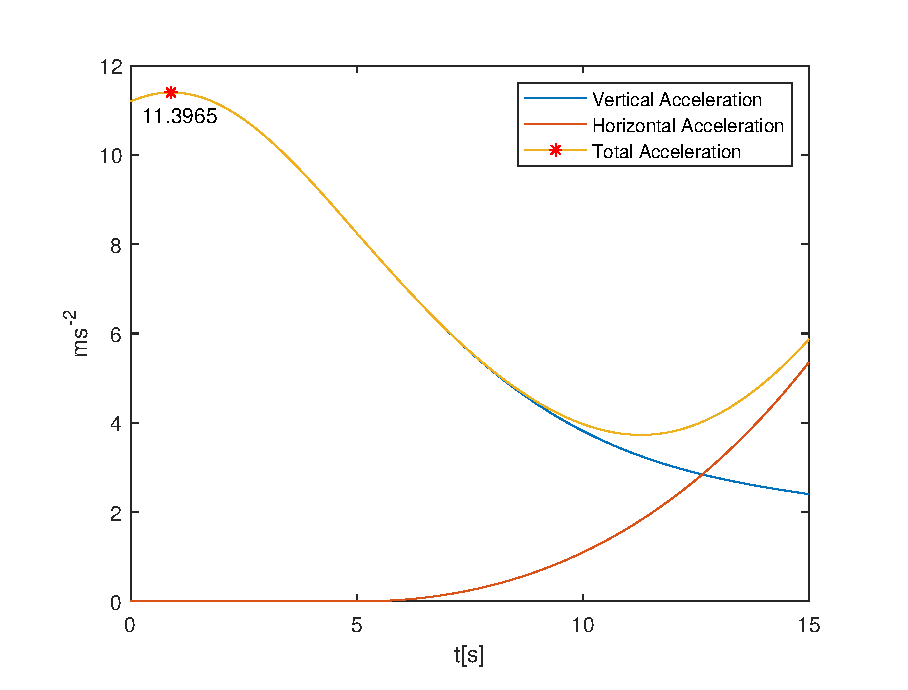
\includegraphics[width=\maxwidth{57.90265930757652em}]{figure_15.eps}
\end{center}

\begin{par}
\begin{flushleft}
Maximum Total Acceleration experienced was $11\ldotp 3965{\mathrm{ms}}^{-2}$
\end{flushleft}
\end{par}


\begin{par}
\begin{flushleft}
\textbf{c) [3 marks] }\textit{Which state variables are important in the linearisation? That is, in which variables is the model non-linear? Provide physical reasoning for the identified non-linearities.}
\end{flushleft}
\end{par}

\begin{par}
\begin{flushleft}
\textbf{Ans. }$x_{\left\lbrack 2,4,6\right\rbrack }$ are related the various velocities of the rocket. The rocket has a constant thrust force with changing mass, experiences drag and also must over come it inertia therefore (and this is seen above) the rocket experiences non-constant acceleration throughout its flight, and thus cannot experience a linear velocity change (and in turn position change). This can be seen represented in the non-linear elements of their equations for their change. ${\dot{\;x} }_{\left\lbrack 1,3,5\right\rbrack } \;$are derived from these and are thus also non-linear.
\end{flushleft}
\end{par}

\begin{par}
\begin{flushleft}
$x_7$ is fuel and undergoes linear depletion. 
\end{flushleft}
\end{par}


\begin{par}
\begin{flushleft}
\textbf{d) [5 marks] }\textit{Linearise the model at the position where it begins its pitch-over manoeuvre }$\left(t=5\right)$\textit{ and plot the rocket’s trajectory when you apply your nominal control signal.}
\end{flushleft}
\end{par}

\begin{par}
\begin{flushleft}
\textbf{Approach: } Form the linearised A, B matrices at the operating points, form a system and run lsim within a modified .m file.
\end{flushleft}
\end{par}

\begin{matlabcode}
DfDx = jacobian(f_sym, [x1, x2, x3, x4, x5, x6, x7])
\end{matlabcode}
\begin{matlabsymbolicoutput}
DfDx = 

\hskip1em $\displaystyle \left(\begin{array}{ccccccc}
0 & 1 & 0 & 0 & 0 & 0 & 0\\
0 & -\frac{x_2 }{250} & 0 & 0 & -\frac{u_1 \,\sin \left(x_5 \right)}{x_7 +1000} & 0 & -\frac{u_1 \,\cos \left(x_5 \right)}{{{\left(x_7 +1000\right)}}^2 }\\
0 & 0 & 0 & 1 & 0 & 0 & 0\\
0 & 0 & 0 & 0 & \frac{u_1 \,\cos \left(x_5 \right)}{x_7 +1000} & 0 & -\frac{u_1 \,\sin \left(x_5 \right)}{{{\left(x_7 +1000\right)}}^2 }\\
0 & 0 & 0 & 0 & 0 & 1 & 0\\
0 & 0 & 0 & 0 & 0 & 0 & -\frac{150\,u_2 }{{{\left(25\,x_7 +20000\right)}}^2 }\\
0 & 0 & 0 & 0 & 0 & 0 & 0
\end{array}\right)$
\end{matlabsymbolicoutput}
\begin{matlabcode}
syms u1 u2
A = subs(DfDx, [x1, x2, x3, x4, x5, x6, x7, u1, u2], 
    ...[clean_X(T==5,:), constant_u1, 0])
\end{matlabcode}
\begin{matlabsymbolicoutput}
A = 

\hskip1em $\displaystyle \left(\begin{array}{ccccccc}
0 & 1 & 0 & 0 & 0 & 0 & 0\\
0 & -\frac{366631709224507}{1759218604441600} & 0 & 0 & 0 & 0 & -\frac{420}{32041}\\
0 & 0 & 0 & 1 & 0 & 0 & 0\\
0 & 0 & 0 & 0 & \frac{4200}{179} & 0 & 0\\
0 & 0 & 0 & 0 & 0 & 1 & 0\\
0 & 0 & 0 & 0 & 0 & 0 & 0\\
0 & 0 & 0 & 0 & 0 & 0 & 0
\end{array}\right)$
\end{matlabsymbolicoutput}
\begin{matlabcode}
DfDu = jacobian(f_sym, [u1, u2])
\end{matlabcode}
\begin{matlabsymbolicoutput}
DfDu = 

\hskip1em $\displaystyle \left(\begin{array}{cc}
0 & 0\\
\frac{\cos \left(x_5 \right)}{x_7 +1000} & 0\\
0 & 0\\
\frac{\sin \left(x_5 \right)}{x_7 +1000} & 0\\
0 & 0\\
0 & \frac{6}{25\,x_7 +20000}\\
-\frac{1}{1000} & -\frac{1}{1000}
\end{array}\right)$
\end{matlabsymbolicoutput}
\begin{matlabcode}
B = subs(DfDu, [x1, x2, x3, x4, x5, x6, x7, u1, u2], 
    ...[clean_X(T==5,:), constant_u1, 0])
\end{matlabcode}
\begin{matlabsymbolicoutput}
B = 

\hskip1em $\displaystyle \left(\begin{array}{cc}
0 & 0\\
\frac{1}{1790} & 0\\
0 & 0\\
0 & 0\\
0 & 0\\
0 & \frac{1}{6625}\\
-\frac{1}{1000} & -\frac{1}{1000}
\end{array}\right)$
\end{matlabsymbolicoutput}
\begin{matlabcode}
A = double(A);
B = double(B);
sys = ss(A,B,[],[]);
figure();
run("q3_linearised_sim.m")
\end{matlabcode}
\begin{center}
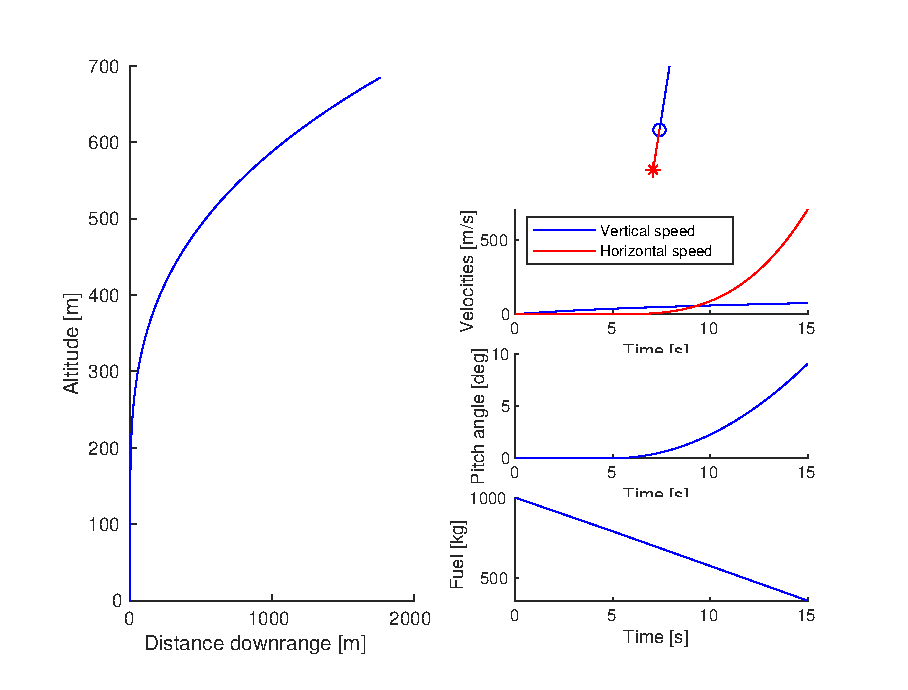
\includegraphics[width=\maxwidth{57.90265930757652em}]{figure_16.eps}
\end{center}
\begin{matlaboutput}
final_angle = 9.0291
\end{matlaboutput}


\begin{par}
\begin{flushleft}
\textbf{e) [5 marks]}\textit{\textbf{ }}\textit{Linearise the model at its final position }$\left(t=15\right)$\textit{ and plot the rocket trajectory when you apply your nominal control signal.}
\end{flushleft}
\end{par}

\begin{matlabcode}
DfDx = jacobian(f_sym, [x1, x2, x3, x4, x5, x6, x7])
\end{matlabcode}
\begin{matlabsymbolicoutput}
DfDx = 

\hskip1em $\displaystyle \left(\begin{array}{ccccccc}
0 & 1 & 0 & 0 & 0 & 0 & 0\\
0 & -\frac{x_2 }{250} & 0 & 0 & -\frac{u_1 \,\sin \left(x_5 \right)}{x_7 +1000} & 0 & -\frac{u_1 \,\cos \left(x_5 \right)}{{{\left(x_7 +1000\right)}}^2 }\\
0 & 0 & 0 & 1 & 0 & 0 & 0\\
0 & 0 & 0 & 0 & \frac{u_1 \,\cos \left(x_5 \right)}{x_7 +1000} & 0 & -\frac{u_1 \,\sin \left(x_5 \right)}{{{\left(x_7 +1000\right)}}^2 }\\
0 & 0 & 0 & 0 & 0 & 1 & 0\\
0 & 0 & 0 & 0 & 0 & 0 & -\frac{150\,u_2 }{{{\left(25\,x_7 +20000\right)}}^2 }\\
0 & 0 & 0 & 0 & 0 & 0 & 0
\end{array}\right)$
\end{matlabsymbolicoutput}
\begin{matlabcode}
syms u1 u2 
A = subs(DfDx, [x1, x2, x3, x4, x5, x6, x7, u1, u2], 
    ...[clean_X(T==15,:), constant_u1, 0])
\end{matlabcode}
\begin{matlabsymbolicoutput}
A = 

\hskip1em $\displaystyle \left(\begin{array}{ccccccc}
0 & 1 & 0 & 0 & 0 & 0 & 0\\
0 & -\frac{3361532086662463}{8796093022208000} & 0 & 0 & -\frac{3360000\,\sin \left(\frac{703690922058203}{70368744177664}\right)}{108641} & 0 & -\frac{268800000\,\cos \left(\frac{703690922058203}{70368744177664}\right)}{11802866881}\\
0 & 0 & 0 & 1 & 0 & 0 & 0\\
0 & 0 & 0 & 0 & \frac{3360000\,\cos \left(\frac{703690922058203}{70368744177664}\right)}{108641} & 0 & -\frac{268800000\,\sin \left(\frac{703690922058203}{70368744177664}\right)}{11802866881}\\
0 & 0 & 0 & 0 & 0 & 1 & 0\\
0 & 0 & 0 & 0 & 0 & 0 & 0\\
0 & 0 & 0 & 0 & 0 & 0 & 0
\end{array}\right)$
\end{matlabsymbolicoutput}
\begin{matlabcode}
DfDu = jacobian(f_sym, [u1, u2])
\end{matlabcode}
\begin{matlabsymbolicoutput}
DfDu = 

\hskip1em $\displaystyle \left(\begin{array}{cc}
0 & 0\\
\frac{\cos \left(x_5 \right)}{x_7 +1000} & 0\\
0 & 0\\
\frac{\sin \left(x_5 \right)}{x_7 +1000} & 0\\
0 & 0\\
0 & \frac{6}{25\,x_7 +20000}\\
-\frac{1}{1000} & -\frac{1}{1000}
\end{array}\right)$
\end{matlabsymbolicoutput}
\begin{matlabcode}
B = subs(DfDu, [x1, x2, x3, x4, x5, x6, x7, u1, u2], 
...[clean_X(T==15,:), constant_u1, 0])
\end{matlabcode}
\begin{matlabsymbolicoutput}
B = 

\hskip1em $\displaystyle \left(\begin{array}{cc}
0 & 0\\
\frac{80\,\cos \left(\frac{703690922058203}{70368744177664}\right)}{108641} & 0\\
0 & 0\\
\frac{80\,\sin \left(\frac{703690922058203}{70368744177664}\right)}{108641} & 0\\
0 & 0\\
0 & \frac{96}{463205}\\
-\frac{1}{1000} & -\frac{1}{1000}
\end{array}\right)$
\end{matlabsymbolicoutput}
\begin{matlabcode}
A = double(A);
B = double(B);
sys = ss(A,B,[],[]);
figure();
run("q3_linearised_sim.m")
\end{matlabcode}
\begin{center}
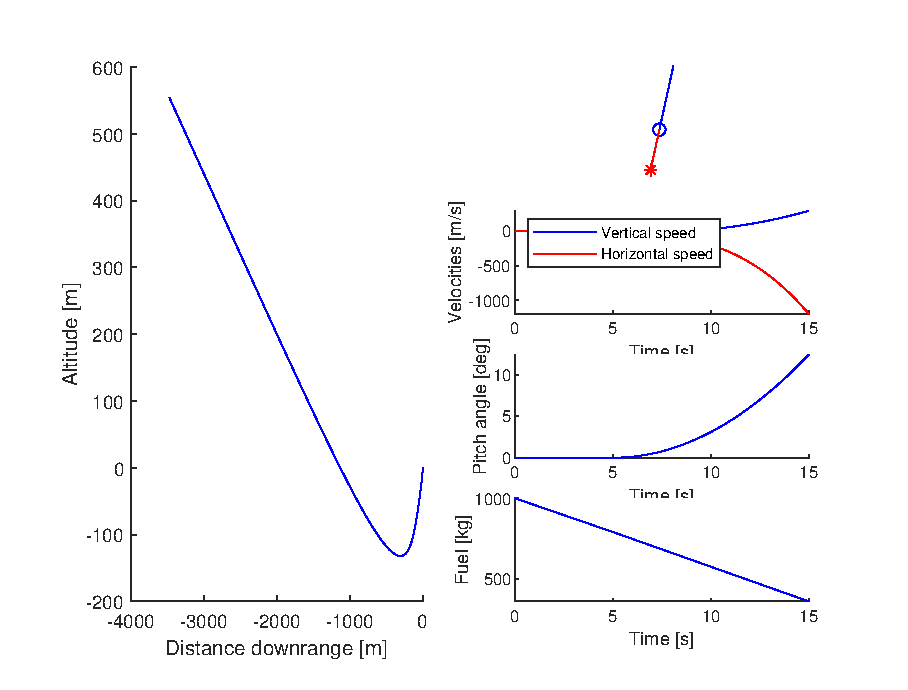
\includegraphics[width=\maxwidth{57.90265930757652em}]{figure_17.eps}
\end{center}
\begin{matlaboutput}
final_angle = 12.3973
\end{matlaboutput}


\begin{par}
\begin{flushleft}
\textbf{f) [5 marks] }\textit{Discuss what you have found from the linearisation, including the differences (if any) between them. What linearisation would you use in a practical implementation of this system?}
\end{flushleft}
\end{par}

\begin{par}
\begin{flushleft}
\textbf{Ans. } Linearising at an operating point of T=5 results in a system that responds very similar to the non-linear simulation with a slight difference in final angle and large difference is horizontal speed and resulting downrange distance, though overall shape of system state progression remains consistent.

At T=15 however, the resulting system is only sparingly close to the "real" system. Fuel and angle are roughly correct but the resulting velocities and positions are wildly incorrect. 

When applying a linearisation to a real world  scenario, choosing an operating point that is within the time you are interested in, though for this system specifically a 1st order approximation still has quite a large divergence.
\end{flushleft}
\end{par}
\end{preview}
\end{document}
